\documentclass[9pt,a4paper]{extarticle}

\usepackage{f1000_styles}

\usepackage{hyperref}

\usepackage[numbers]{natbib}

% include \verb macros in \caption of figures

% http://tex.stackexchange.com/a/8814

\usepackage{cprotect}

\begin{document}

\pagestyle{front}

\title{Creating and sharing reproducible research code the workflowr
way}

\author[1]{John D. Blischak}

\author[1,2]{Peter Carbonetto}

\author[1,3]{Matthew Stephens}

\affil[1]{Department of Human Genetics, University of Chicago}

\affil[2]{Research Computing Center, University of Chicago}

\affil[3]{Department of Statistics, University of Chicago}

\maketitle

\thispagestyle{front}

\begin{abstract}

\# Note: Abstract can be as long as 300 words.

The workflowr R package helps scientists create code and results that
are organized and reproducible, well-documented, and more readily
communicated with other scientists. Workflowr provides a core set of
commands that can be easily integrated into research practice to make
programming projects more reproducible and accessible. The core
workflowr commands implement four key features of reproducible code: (1)
automatic project structure intended to promote better organization of
data, code and results; (2) packaged code and results that are assigned
a uniquely identifiable label, then incorporated into a project
development history to document progress; (3) automated "reproducibility
checks" that accompany each packaged collection of code and results; and
(4) tools to facilitate online sharing of project code and results. To
achieve these reproducibility features, workflowr integrates version
control (Git), literate programming tools (knitr, R Markdown), and
static Web hosting (e.g., via GitHub or GitLab Pages) into a simple and
uniform R interface. Our aim is to encourage \textit{all} scientists,
regardless of background,to organize and share their reproducible
research code. The workflowr R package is open source and available on
CRAN, with full documentation and source code available at
https://github.com/jdblischak/workflowr.

\end{abstract}

\section*{Keywords}

reproducibility, open science, workflow, R, interactive programming,
literate programming, version control

\clearpage

\pagestyle{main}


\section*{Introduction}

A central tenet of the scientific method is that results should be
independently verifiable --- and, ideally, extendible --- by other
researchers [ref]. As computational methods play an increasing role in
many disciplines, key scientific results are very often produced by
computer code. Verifying and extending such results requires that the
code be ``reproducible''; that is, it can be accessed and run, with
outputs that can be corroborated against published articles
\cite{Buckheit1995, Gentleman2005, Peng2011, Ince2012, Morin2012,
Sandve2013, Easterbrook2014, Stodden2016, Lowndes2017}. Unfortunately,
this ideal is not usually achieved in practice; most scientific articles
do not come with code that can reproduce their results
\cite{Ioannidis2009, Ioannidis2014, Stodden2018}.

There are many barriers to sharing reproducible code and corresponding
computational results. One barrier is simply that keeping code and
results sufficiently organized and documented is difficult—it is
burdensome even for experienced programmers who are well-trained in
relevant computational tools such as version control (discussed later),
and even harder for the many domain scientists who write code with
little formal training in computing and informatics \cite{Wilson2014b}.
Further, modern interactive computer environments (e.g., R, python),
while greatly enhancing code development \cite{Findler2002}, also make
it easier to create results that are irreducible. To take one example,
it is all too easy to run interactive code without recording or
controlling the seed of a pseudo-random number generator, or generate
results in a ``contaminated'' environment that contains objects whose
values are critical but unrecorded. Both these issues can lead to
results that are difficult or impossible to reproduce. Finally, even
when analysts produce code that is reproducible in principle, sharing it
in a way that makes it easy for others to retrieve and use (e.g., via
GitHub or Bitbucket) involves technologies that many scientists are not
familiar with \cite{Stodden2018}.

In light of this, there is a pressing need for easy-to-use interactive
programming tools to help analysts keep code and results organized and
reproducible, document progress, and disseminate code and results to the
scientific community. We have developed an open source R \cite{R2019}
package, "workflowr", to help address this need. The workflowr package
aims to instill a particular "workflow"—a sequence of steps to be
repeated and integrated into research practice—that help make projects
reproducible and accessible. To achieve this, workflowr integrates four
key tools of reproducible code development: (1) version control
\cite{Loeliger2012, Chacon2014}; (2) literate programming
\cite{Xie2015}; (3) automatic "reproducibility safeguards”—simple
checks, like setting and recording the random number seed, that improve
code reproducibility; and (4) static website creation from R source
code. These features exploit powerful existing tools, whose mastery
would take considerable study. However, the workflowr interface is
designed to be simple, so that learning it does not become another
barrier in itself, and novice users can quickly enjoy its many benefits.
By simply following the workflowr workflow, R users can create projects
whose results and figures are easily accessible on a static website ---
therefore conveniently shareable with collaborators by sending them a
URL --- and accompanied by source code and reproducibility safeguards.
The Web-based interface, updated with version control, also makes it
easy to browse the project history --- including previous versions of
figures, other results, and the code used to produce them. And all this
is possible with minimal experience in version control systems and Web
technologies.

The workflowr package builds on several software technologies and R
packages, without which this work would have not been possible. First,
workflowr builds on the invaluable R literate programming system
provided by the knitr and rmarkdown packages \cite{}, which in turn
build on pandoc \cite{}, the "Markdown" markup language [ref], and
various Web technologies such as Cascading Style Sheets and Bootstrap
[ref]. Workflowr augments rmarkdown with additional features such as the
reproducibility safeguards, and adds integration with Git \cite{}.
Although Git was originally intended to support large-scale, distributed
software development \cite{}, in workflowr it is primarily used for a
different purpose: to record, and provide access to, the development
history of a project. Workflowr also uses another feature of
Git—"remotes"—to enable collaborative project development across
multiple locations, and to help users create browsable projects on the
internet via integrations with popular online services such as GitHub
Pages and GitLab Pages. These features are implemented via the R package
git2r, which provides an interface to the libgit2 C library. Finally,
beyond extending the R programming language, workflowr also integrates
seamlessly with the popular RStudio interactive development environment.

In addition to these tools on which workflowr directly builds, there are
many other related tools that directly or indirectly advance open and
reproducible data analysis. A comprehensive review of such tools is
beyond the scope of this article, but we note that many of these tools
are complementary to workflowr in that they tackle aspects of
reproducibility that workflowr currently leaves to the user: for
example, management of computational environments and/or dependencies,
locally or on "the cloud" (e.g., conda, Homebrew, Singularity, Docker,
Kubernetes, packrat, checkpoint, switchr, Binder, rsuite); development
and management of computational pipelines (e.g., GNU Make, Snakemake,
drake); managing or archiving data objects (e.g., archivist, cacher,
Dryad, Zenodo); and distribution of open source software (e.g., CRAN,
Bioconductor, Bioconda). Most of these tools or services could be used
in combination with workflowr. Lastly, we note that there are many other
useful tools whose features overlap with those of workflowr, which would
make it difficult or impossible to use in combination. These include
standalone software tools such as ActivePapers
\url{https://www.activepapers.org/}, adapr \cite{Gelfond2018},
ProjectTemplate, rrtools, Sumatra
\url{https://pythonhosted.org/Sumatra/}, as well as online computing
platforms such as Code Ocean, Gigantum, and The Whole Tale. We document
similar R packages at
\url{https://github.com/jdblischak/ctv-project-workflows}.

The workflowr R package is available from CRAN
(https://cran.r-project.org/package=workflowr) and GitHub
(https://github.com/jdblischak/workflowr), and is distributed under the
flexible open source MIT license. Extensive documentation, tutorials and
user support can be found on the GitHub site. In the remainder of this
article, we describe the workflowr interface, explain its design, and
give examples illustrating how workflowr is used in practice (see "Use
Cases").


\section*{Methods}

The workflowr R package makes data analysis projects more organized,
tracked, reproducible, and shareable. The R package and its dependencies
are straightforward to install, while also being highly customizable for
more experienced users. In the following sections, we give an overview
of the features of the workflowr R package, and describe their
implementation. For step-by-step instructions on starting a workflowr
project, see the
\href{https://jdblischak.github.io/workflowr/articles/wflow-01-getting-started.html}{"Getting
started with workflowr"} vignette.

\subsection*{Operation}

\subsubsection*{Organizing files and results}



\begin{figure}

\centering

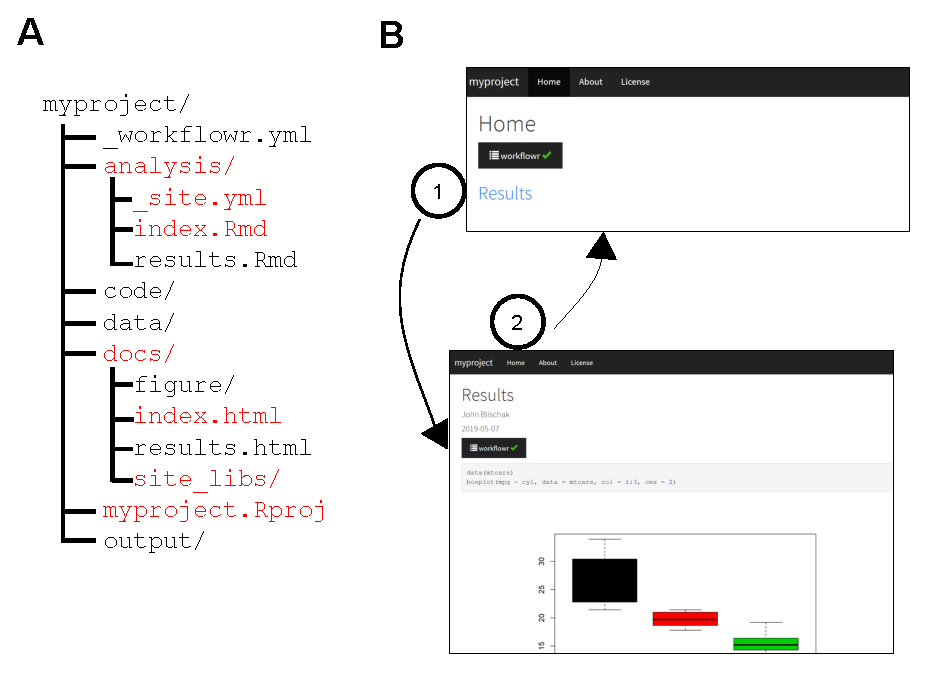
\includegraphics[width=0.8\textwidth]{figures/wflow-fig-1-v01.eps}

\cprotect\caption{\label{fig:organized}

The workflowr package organizes files and results. A) The function
\verb|wflow_start()| populates a new project directory with all the files
needed to begin a workflowr project. The default directory structure
encourages users to organize their files as the project progresses (this
is only a suggested structure, and users may change the names of many of
the files and directories as they see fit). Files that are required by
workflowr are shown in red. B) The results are organized into a website
which is stored in the "docs" folder. The use of hyperlinks allows
readers to efficiently browse and access the results. The example
screenshots demonstrate how to navigate a workflowr website. Clicking on
a hyperlink in the main page (1) takes you to a webpage with results.
Then clicking on the Home hyperlink (2) in the navigation bar returns
you to the main page.

}

\end{figure}

One of the aims of workflowr is to promote peer review of data analyses,
which requires that shared code and results be organized and accessible.
However, without the proper tool to facilitate this, a typical project
will evolve to an unstructured collection of files, resulting in
frustration and an ineffective peer review process.

The workflowr package provides simple tools to facilitate staying
organized from the outset. The function \verb|wflow_start()| populates a new
project directory with suggested subdirectories, scripts, and
configuration files for a data analysis (Figure \ref{fig:organized}A). By default, the
subdirectories include: analysis/ for scripts that produce results such
as figures and tables; docs/ for storing the webpages that make up the
workflowr website; code/ for longer running scripts, compiled code
(e.g., C++), and other source code supporting the data analyses; data/
for raw data files; and output/ for processed data files and other
outputs generated by the scripts and analyses. Importantly, this setup
is flexible and configurable; only two of these directories are
required, \verb|analysis/| and \verb|docs/|, and both of these
directories can be renamed later.

Beyond data and source code, it is also important to organize
results—consider that most scientific publications have a results
section that conforms to a standard logical structure. However, the
sequential structure of a scientific paper is not appropriate for an
ongoing investigation or exploratory data analysis; for more typical
uses of workflowr, it is more appropriate to have a flexible,
non-sequential layout that can be easily modified and expanded on, and
so that a reader can quickly jump to relevant parts of the analysis.
HTML is very well suited for this purpose; it is specifically designed
to quickly access relevant information in the same document or in
another document. In R, the knitr and rmarkdown packages automate
generation of HTML from R Markdown. In the workflowr package, the
\verb|wflow_build()| function provides this service.

Once a data analysis has been implemented in an R Markdown file,
\verb|wflow_build()| will do the work of packaging the code and results into a
single HTML webpage. Webpages are easily revised after changes are made
to the analysis, again by using the \verb|wflow_build()| function. Thus, a
typical workflowr use will involve iterating between revisions to the R
Markdown analyses and calls to \verb|wflow_build()|. \textit{The primary output
of workflowr is a website organizing the results generated by R Markdown
analyses} (Figure \ref{fig:organized}B).

\subsubsection*{Tracking development history with version control}

As an analysis project progresses, many versions of the results are
produced as existing results are scrutinized, decisions are made,
mistakes are fixed, and new data sets are considered. Keeping track of
this evolution is important for documenting this progress and retracing
the development of an analysis. Without version control, documenting the
analysis history by copying code and results whenever an important
change is made—typically resulting in a large collection of files with
names such as \verb|results-v2-final_final.pdf| and
\verb|anova_analyses_before_adding_new_samples.R|—is not only tedious,
but also error-prone, and makes it difficult to communicate changes to
collaborators.

There is now a much better way to keep track of the evolution of your
analysis: using the version control system, Git. Git presents two
challenges, however. First, since Git was designed for large teams of
software engineers to collaborate on large-scale software projects, the
features and documentation are overly complex for any researcher unless
they are already an experienced computer scientist or software engineer.
This steep learning curve can discourage researchers from using Git for
their projects. Second, Git was originally intended to manage code, and
was not envisaged as a tool for tracking development of a data analysis
project—consider that the researcher will want to track not only the
source code and data, but also the results generated by the code and
data.

To address these two challenges, we developed workflowr with two key
design points in mind.

Our first design decision was to provide a simple interface to the
subset of Git commands that are most essential for tracking a data
analysis project. This means that a researcher using workflowr can adopt
Git from the very beginning of their project without having to be
comfortable with the Git command-line interface.

Second, we designed workflowr so that it manages source code files (R
Markdown) differently from the results files (webpages and figures).

While these two decisions influenced the way we designed the entire
workflowr package, the impact of these two decisions are best
illustrated by describing the operation of \verb|wflow_publish()|, which is one
of the key functions in the workflowr interface. This function performs
three key steps, illustrated in Figure \ref{fig:publish}:

1. Commit source: Commit the R Markdown source file to the Git
repository, and record the "Secure Hash Function"—a hexadecimal
sequence, often abbreviated as "SHA1", that uniquely identifies the
commit in the Git repository.

2. Render results: Execute the source code to generate the results, and
compile the results into an HTML file. Workflowr embeds the HTML with
the SHA1 generated in Step 1.

3. Commit results: Commit the HTML and figure files generated in Step 2.

The three-step \verb|wflow_publish()| procedure guarantees that each new
collection of results—stored in an HTML file and accompanying figure
files—is produced by a unique and identifiable version of an R Markdown
source file.

The sequence of Git commands and other operations are executed behind
the scenes, so that the user only needs to make a simple call to
\verb|wflow_publish()|. We have also implemented many checks and extensive
error handling to make sure that the Git repository and R environment
are in an acceptable state for committing the results. (When there are
issues, workflowr provides guidance on how to fix these issues).

Another key benefit of the \verb|wflow_publish()| three-step procedure is that
it provides a \textit{workflow} for using Git in a data analysis
project. Even people who are comfortable with Git may be unsure how to
use Git for a data analysis—what files to commit and how often? Although
workflowr does not address every Git-related question, it does provide a
Best Practice commit protocol for a data analysis:

1. Every commit to an (R Markdown) analysis file is paired with a commit
to the results file generated by that R Markdown file.

2. \textit{An analysis file is only committed if it successfully runs};
upon failure, \verb|wflow_publish()| aborts, and neither code nor results are
committed to the Git repository. (workflowr cannot stop someone from
committing code that does not work, but it can at least encourage this
practice through the workflowr interface.)



\begin{figure}

\centering

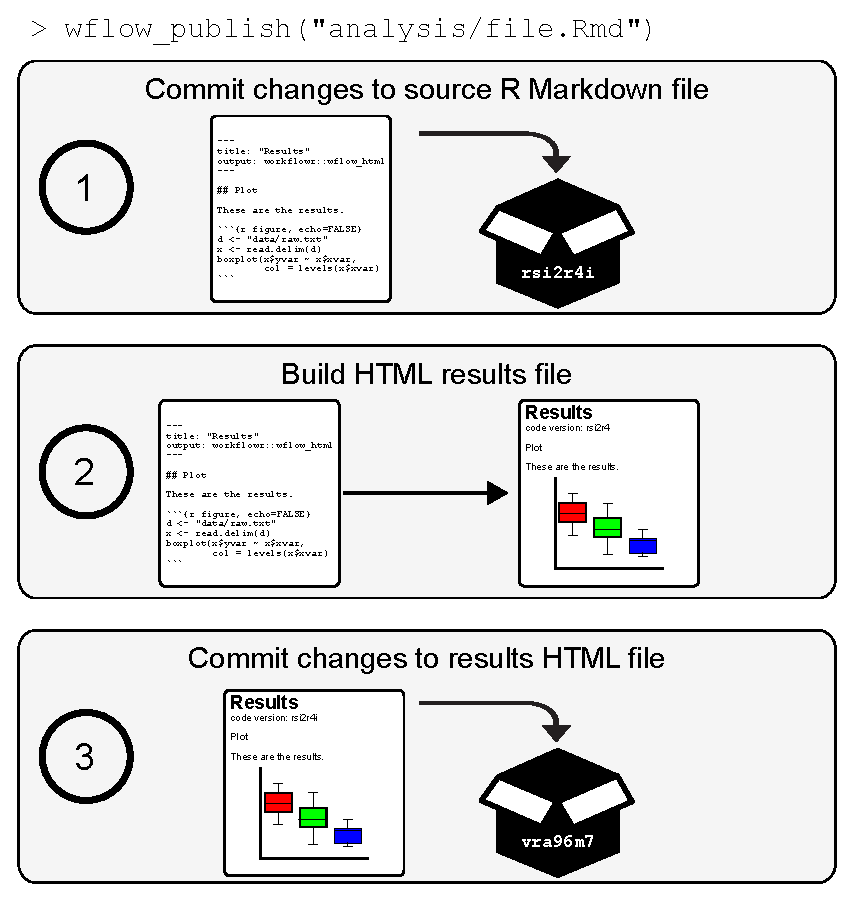
\includegraphics[width=0.8\textwidth]{figures/wflow-fig-2-v01.eps}

\cprotect\caption{\label{fig:publish}

The function \verb|wflow_publish()| versions the source and results files. The
function \verb|wflow_publish()| performs a 3 step process to ensure that the
result HTML file is always created from a specific version of the source
R Markdown file. (1) The first step commits the changes to the source R
Markdown file. (2) The second step builds the results HTML file from the
source R Markdown file. This ensures that the results were generated
from this exact version of the R Markdown file. Furthermore, the unique
version of the Git repository is inserted directly into the HTML file to
facilitate transparency. (3) The results HTML file (and any related
figure files) are committed to the Git repository. Thus the results of
the analysis are versioned in addition to the source code.

}

\end{figure}

One way to view workflowr is as an rmarkdown-aware version control
system. To track the development of the R Markdown files, workflowr
assigns a status to each one (Figure \ref{fig:versioned}). These statuses are used
internally, but can also be reported to the user with \verb|wflow_status()|.
Specifically, the status of each R Markdown file corresponds not only to
its own status in Git but also its corresponding HTML file. A “scratch”
R Markdown file is one that is not yet being tracked with Git. An
“unpublished” R Markdown files is one that is tracked by Git, but its
accompanying HTML file is not. A “published” R Markdown file is one that
is tracked by Git as well as its accompanying HTML file. Furthermore,
each “published” R Markdown file has a substatus. If no changes have
been made to the R Markdown file since its HTML file was last published,
it is “up-to-date”. In contrast, if an R Markdown file has been modified
since the last time its HTML file was published, it is “modified”. The
function \verb|wflow_status()| reports all the R Markdown files which have the
status “scratch”, “unpublished”, or “modified”, and recommends the user
to publish the results with \verb|wflow_publish()|.



\begin{figure}

\centering

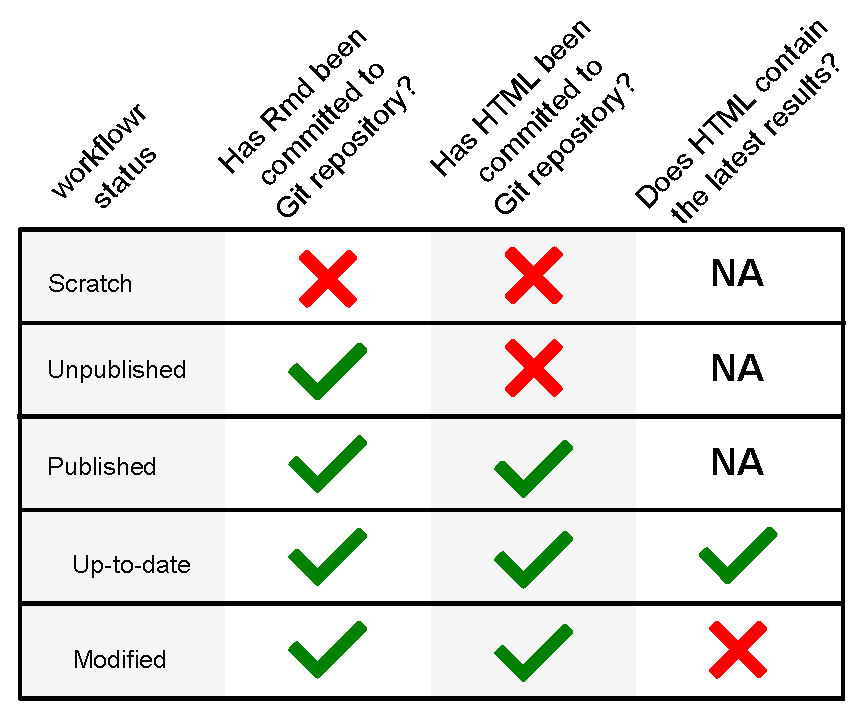
\includegraphics[width=0.8\textwidth]{figures/wflow-fig-3-v01.eps}

\cprotect\caption{\label{fig:versioned}

The workflowr package is an R Markdown aware version control system. The
function \verb|wflow_status()| assigns a status to each R Markdown file in the
project based on the its Git status and that of its corresponding HTML
file.

}

\end{figure}

\subsubsection*{Reproducing past results}

Reproducing computational results is challenging, even for the original
author. Therefore it is important to follow best practices for
reproducible research \cite{Sandve2013, Wilson2014a, Wilson2017}.
Unfortunately not only is this list of best practices daunting for
novices to incorporate, it is also easy for experienced practitioners to
mistakenly forget an important step. The philosophy of workflowr is to
automate as many reproducibility steps as possible so that researchers
can focus on their analysis. Furthermore, workflowr embeds a report of
which reproducibility checks passed or failed at the top of each file,
so that the original author as well as any readers know which
reproducibility safeguards were applied to each analysis.

When executing the code in an R Markdown file with \verb|wflow_build()| or
\verb|wflow_publish()|, workflowr automatically implements multiple
reproducibility safeguards (Figure \ref{fig:reproducible}). First, it starts a new R process
to execute the code. This avoids any unpredictable issues arising from
objects defined in the user’s current R session (e.g. if a critical
variable was only defined in the current session, the code in the file
would execute, but then fail in any future session). Second, it sets a
seed for the pseudo-random number generator before execution, so that
analyses that rely on random numbers always return the same result.
Third, it records information on the current operating system, R
version, and package versions that were used to produce the results.
Lastly, workflowr performs reproducibility checks and inserts a report
at the top of the HTML page. As long as the user does not disable the
automated steps above, each analysis will pass these checks. In
addition, workflowr checks and reports the current status of the Git
repository and other factors important for reproducibility.



\begin{figure}

\centering

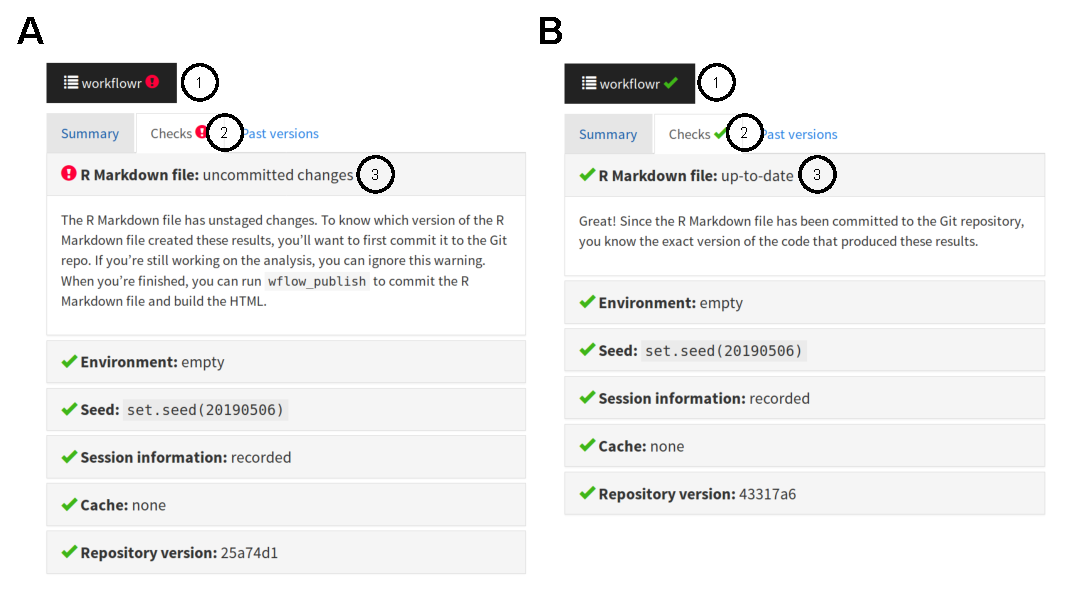
\includegraphics[width=0.8\textwidth]{figures/wflow-fig-4-v01.eps}

\cprotect\caption{\label{fig:reproducible}

The workflowr report describes the reproducibility checks. A) There is a
button at the top of each HTML file that contains the workflowr report.
If any of the reproducibility checks failed, it will display a red
warning symbol. Clicking on the button (1) reveals the full workflowr
report with multiple tabs. Clicking on the tab Checks (2) lists all the
checks that passed or failed. Clicking on any of these (3) produces more
explanatory text. In this example, the R Markdown file has uncommitted
changes (this is fine during active development of the analysis, but
once it is ready to share, it needs to be committed). The text suggests
running \verb|wflow_publish()| to remove the warning. B) If all the workflowr
reproducibility checks pass, then the workflowr button will instead
display a green checkmark. This time, clicking the individual
reproducibility check (3) will explain why it was important that the
check was performed.

}

\end{figure}

\subsubsection*{Sharing results online}

The version-controlled results website created by workflowr is a
self-contained static website. This means that the website subdirectory
can be copied to any web server to host the website online. Once online,
a user can share the URL with collaborators and colleagues and also
include it in the Methods section of a paper.

Because a workflowr project is already a Git repository, the easiest
option for hosting the website is to take advantage of the free static
web hosting provided by Git hosting

services (e.g. GitHub Pages or GitLab Pages). Workflowr provides the
functions \verb|wflow_use_github()| and \verb|wflow_use_gitlab()| that will perform
all the one-time local steps to prepare the project for using GitHub or
GitLab, respectively. After a user creates a new Git repository on the
online platform, she can upload the project from their local machine
with \verb|wflow_git_push()|.

An important goal of the workflowr website is to allow any reader to
take advantage of version control without having to write or execute any
code. In addition to the reproducibility report, workflowr also
automatically inserts links to every past version of the R Markdown
file, the HTML file, and any figure files. For example, if a
collaborator wants to download a specific version of a figure from six
months ago, she could do this with a few clicks on the workflowr
website.

\subsubsection*{Installation}

The workflowr software is available on CRAN and can be downloaded from
within the R console with \verb|install.packages("workflowr")|. It is
regularly comprehensively tested on all major operating systems (Linux,
macOS, Windows), and will work with R version 3.2.5 or later. Because
workflowr uses the rmarkdown package to build the HTML pages, it
requires the document conversion software pandoc to be installed. The
easiest method for R users to install pandoc is to install RStudio,
which automatically installs it. Note that installation of Git is
optional, but is recommended if users need to perform more complex Git
operations.

\subsubsection*{Customization}

A workflowr website is designed to be customizable. Common HTML styling
settings from the rmarkdown package can be configured in the file
\verb|analysis/_site.yml|. Workflowr-specific settings, e.g. the seed to
set or which directory to execute the code in, can be configured in the
file \verb|_workflowr.yml|.

\subsubsection*{Miscellaneous}

The workflowr package aims to reduce the difficulty with working
directories, especially when working with R Markdown files. First, all
the workflowr commands can be run from within any subdirectory of the
workflowr project, and they will behave the same. Second, by default all
the R Markdown files are executed from the root of the workflowr
project, even though the files themselves are located in a subdirectory.
This fixes a common pain point for new R Markdown users, when they test
their code in one directory but then the file executes in the directory
where it is saved.

\subsection*{Implementation}

\subsubsection*{Organizing files and results}

The function \verb|wflow_start()| populates the project directory using
pre-defined template files. Furthermore, it uses the R package glue to
insert relevant variables, e.g. the name of the project, directly into
the newly created files.

The function \verb|wflow_build()| builds a website from a collection of R
Markdown files using the function \verb|render_site()| from the rmarkdown
package. The function \verb|render_site()| downloads and links all the
necessary CSS and JavaScript files to create a responsive website with a
navigation bar (specifically it uses the Bootstrap framework). The
website settings can be configured in the file
\verb|analysis/_site.yml|, e.g. the links in the navigation bar and the
path to the website directory. Similar to other R packages that extend
rmarkdown (e.g. bookdown), workflowr provides a custom site generator,
\verb|wflow_site()|, to modify this process. The most noticeable difference
from the default is that the generated website files (HTML, CSS,
JavaScript) are moved from \verb|analysis/| to \verb|docs/| instead of
copied, which avoids duplication and reduces the number of files per
subdirectory.

\subsubsection*{Tracking development history with version control}

The workflowr functions use the R package git2r to run Git commands. The
git2r package is a wrapper around libgit2, a minimal C implementation of
Git.

The function \verb|wflow_status()| determines the status of each R Markdown
file in the project by comparing its Git status to the Git status of its
HTML file. Using Git’s nomenclature, a “scratch” R Markdown file is
uncommitted, an “unpublished” R Markdown file is committed but not its
HTML, a published R Markdown file and its HTML file are both committed,
and a modified R Markdown file has any changes (they can be unstaged,
staged, or committed) that were made since the last time its HTML file
was committed (Figure \ref{fig:versioned}).

\subsubsection*{Reproducing past results}

Workflowr uses the R package callr to start a new R process and execute
the code. Workflowr injects code chunks and the reproducibility report
into the file using a custom output format, \verb|wflow_html()|, which extends
the output format \verb|html_document()| from the rmarkdown package. In this
way users gain the benefits of workflowr’s reproducibility features
while still being able to use the latest customization features
implemented in rmarkdown (e.g. table of contents, folding of code
chunks, etc.). The seed is set by inserting a code chunk at the start of
the file to run the base R function set.\verb|seed()|. The session information
is recorded at execution by inserting a code chunk at the end of the
file to run the base R function sessionI\verb|nfo()|.

\subsubsection*{Sharing results online}

The functions \verb|wflow_use_github()| and \verb|wflow_use_gitlab()| set the remote
Git repository (i.e. git remote add origin URL, via \verb|wflow_git_remote()|)
and add a link to the source code repository into the navigation bar.
Additionally, \verb|wflow_use_gitlab()| configures GitLab Pages via the file
.gitlab-ci.yml (unfortunately setting up GitHub Pages must be done
manually because it is not currently exposed via the GitHub API).
Neither function automatically creates the repository online. (This
would require the user to create a personal access token, and we decided
it is easier for users to leave this once-per-project action as a manual
step.)

The links to past versions of the files are inserted by \verb|wflow_html()|.
This requires that the user has set a remote Git repository, which
workflowr uses to determine the URL to past versions. Links to past
versions of the R Markdown file (or figure files) load that file at the
given Git commit on GitHub or GitLab. Links to past versions of the HTML
pages use the service raw.githack.com, which properly renders the HTML
file for convenient viewing (a direct link to the file on GitHub or
GitLab would display the raw HTML).

\subsubsection*{Installation}

Installation of the workflowr package itself is easy because it is
available for download from CRAN. The user does not need to install Git
because workflowr uses the minimal Git library libgit2, via the R
package git2r. Most workflowr users also use RStudio, which installs
pandoc. Advanced users can directly install Git and pandoc for more
control and flexibility if desired.

\subsubsection*{Customization}

The settings specified in \verb|analysis/_site.yml| are passed to the
function \verb|html_document()| from the rmarkdown package. The settings in
\verb|_workflowr.yml| are read by \verb|wflow_html()| when implementing the
reproducibility features. For example, instead of recording the session
information with sessionI\verb|nfo()|, a user can add the line
\verb|sessioninfo: "devtools::session_info()"| to \verb|_workflowr.yml|
to use the version from the devtools package.

\subsubsection*{Miscellaneous}

The workflowr commands can be invoked from any project subdirectory
(similar to how Git commands work). This is achieved by searching for
the RStudio project file at the root of the project using the R package
rprojroot.

The workflowr package can be configured to execute the R Markdown files
in a different directory from where they are saved. This execution
directory is controlled by the rmarkdown option \verb|knit_root_dir|,
which is set in \verb| _workflowr.yml| and read by \verb|wflow_html()| before
executing the code. By default, new projects execute the R Markdown code
chunks in the root directory.


\section*{Use cases}

A workflowr website is useful for any situation in which a user wishes
to organize and share reproducible computational results. The most
common use cases include:

\begin{itemize}

\item \textbf{Single-user research website:} A researcher working solo
on a project can track her intermediate results and easily share the
latest results by sending the URL for a given analysis to her
colleagues.

\begin{itemize}

\item
\href{https://davismcc.github.io/fibroblast-clonality/}{fibroblast-clonality}

\item \href{https://jean997.github.io/rccSims/}{rccSims}

\item
\href{https://brimittleman.github.io/threeprimeseq/}{threeprimeseq}

\item \href{https://lsun.github.io/truncash/}{truncash}

\end{itemize}

\item \textbf{Collaborative research website:} Because workflowr uses
the version control system Git, multiple researchers can collaborate on
a research project using Git and a Git-hosting site (e.g. GitHub,
GitLab, etc.). By using workflowr, they will know the results of their
collaborator’s analyses are reproducible by reading the workflowr
report.

\begin{itemize}

\item \href{https://jdblischak.github.io/fucci-seq/}{fucci-seq}

\item
\href{https://jdblischak.github.io/singlecell-qtl/}{singlecell-qtl}

\end{itemize}

\item \textbf{Course website:} Any course or workshop that aims to teach
computational methods can benefit from workflowr. The research website
makes it easy to disseminate the content to the learners, and the
reproducibility report confirms that they should be able to run the code
themselves.

\begin{itemize}

\item \href{https://annakrystalli.me/intro-r-gis/}{intro-r-gis}

\item
\href{https://xiangzhu.github.io/stanford-stats141/}{stanford-stats141}

\end{itemize}

\end{itemize}


\section*{Summary}

The workflowr R package aims to lower the barrier to open and
reproducible computational results. It is simple to install, easy to
learn since it builds on the popular R programming language and R
Markdown format for literate programming, and extremely customizable
should users desire to learn the intricacies of Git, HTML, and CSS.

The first official release of workflowr was made available for download
from CRAN in April 2018. The core functionality has been stable and will
continue to be. In the future, we plan to implement the following
enhancements:

\begin{itemize}

\item Provide documentation and helper functions to support hosting the
workflowr website on additional platforms. Because it is a static
website, it could be hosted on many different platforms such as GitLab,
Netlify, Heroku, etc.

\item Create a centralized website for registering and sharing workflowr
projects. In order to better promote open science, we would like to make
it easier for other interested researchers to discover existing
workflowr projects.

\item Implement basic support for small pipelines. Currently the only
way to have workflowr execute R Markdown files in a specific order is to
name them in alphanumeric order. In the future, we plan to make it
possible to specify which R Markdown files depend on each other.
However, since it will still be focused only on R Markdown files, users
will still be encouraged to use dedicated pipeline software to build
complex data analysis pipelines.

\end{itemize}

While workflowr aims to facilitate reproducible research, it is of
course not foolproof. Major limitations include 1) versioning of large
data files, 2) managing the computational environment, and 3) willful
tampering. The workflowr package ensures that each HTML results file was
created from a specific, known version of the corresponding R Markdown
file, which is critical for reproducibility. However, if any imported
data files are not versioned by Git (or are out-of-date), then the
results will not be reproducible. This is mainly an issue for large data
files. Users are recommended to use Git LFS or similar software to
version large data files. Managing software dependencies is complex, and
there exist many solutions ranging from language-specific package
managers (e.g. packrat) to operating-system-level virtualization (e.g.
Docker). Instead of prescribing one solution over others, the workflowr
package simply records the session information that produces each
result, and otherwise leaves each user to decide how best to manage this
complexity. Lastly, the development history recorded by Git can be
edited. Thus while useful for transparency, it cannot be considered an
immutable record (e.g. like that provided by a blockchain).


\section*{Data availability}

Not applicable


\section*{Software availability}

The workflowr software is open-source and available at the links below:

\begin{enumerate}

\item CRAN: \url{https://cran.r-project.org/package=workflowr}

\item Source code: \url{https://github.com/jdblischak/workflowr}

\item Documentation: \url{https://jdblischak.github.io/workflowr/}

\item Zenodo: \url{https://zenodo.org/badge/latestdoi/75893305}

\item License: \href{https://choosealicense.com/licenses/mit/}{MIT}

\end{enumerate}


\section*{Author Contributions}

JDB: Conceptualization, Software

PC: Software

MS: Conceptualization, Funding Acquisition, Supervision


\section*{Competing interests}

No competing interests were disclosed.


\section*{Grant information}

This work was supported by the Gordon and Betty Moore Foundation [Grant
number \#4559].

The funders had no role in study design, data collection and analysis,
decision to publish, or preparation of the manuscript.


\section*{Acknowledgments}

We are very thankful to workflowr
\href{https://github.com/jdblischak/workflowr/graphs/contributors}{contributors}
for helping improve the package. We are also grateful for workflowr
users for testing the package and providing feedback---thanks especially
to \href{https://github.com/LSun}{Lei Sun},
\href{https://github.com/xiangzhu}{Xiang Zhu},
\href{https://github.com/NKweiwang}{Wei Wang}, and other members (past
and present) of the Stephens lab.

We are also grateful to the authors and contributors of the many great
open source packages that the workflowr package uses. Especially
critical for workflowr are the R packages
\href{https://cran.r-project.org/web/packages/git2r/index.html}{git2r},
\href{https://github.com/yihui/knitr}{knitr}, and
\href{http://rmarkdown.rstudio.com/}{rmarkdown}.


{\small\bibliographystyle{unsrtnat}

\bibliography{references}}

\end{document}
